\section{Entity Relationship Diagram}
\subsection{Entities}
We will have six entities: user, post, question, answer, comment, and topic.

A user is an individual writing a post on Ask Us. The user entity will have five attributes: ID, username, email, password, and points. A user's points are the sum of all the points of all their posts. ID will be the primary key.

A post is anything a user writes. This can either be a question, answer, or comment. The post entity will only have an ID, which is the primary key. The purpose of this entity is mainly so that comments can have their parent post be of any type. (We can comment on questions, answers, and even other comments.)

Questions, answers, and comments will all have the following attributes, aside from the ones we specify below. They will have a body, which is the main text that makes up that post. They will also have a count of the points that they have been awarded by users. They will also have a timestamp which will be the exact date and time a post was made.

The question entity has one other attribute called title, aside from the attributes listed above. Since it is a weak entity, its primary key is the post's ID.

The answer entity has a boolean attribute called accepted, apart from the attributes it has in common with the other post types. Similarly, since it is a weak entity, its primary key is the post's ID.

A comment is typically a short piece of text that a user writes beneath any kind of post. A comment itself has no other attributes, other than the ones above. Once again, since it is a weak entity, its primary key is its post's ID.

A topic is a way for users to categorize their questions, thus getting better targeted responses. A user can also follow a topic of interest. The topic entity will have three attributes: ID, username, and description. ID will once again be the primary key.

\subsection{Relations}
A user can `follow' a topic. In this relation, there can be many topics a user can follow, but it is not mandatory for a user to follow any topic. In the same light, topics can be followed by any number of users.

A user is related to the posts that they write. In this relation, the user can write anywhere from many to no posts. However, a post must be written by exactly one user.

A user is also related to a post by voting on it. The vote relation is a many to many relation, in that a user can vote on many to no posts and a post can be voted on by many to no users.

The comment entity has two relations with the post entity. One relation is called belongs to. This relation represents the fact that a specific comment has a parent post (which may also be a comment). A post can optionally have many comments, but a comment must be a child of exactly one post.

The other relation is an inheritance relation. It is an identifying relation, and is labelled `is a' in figure \ref{erd2}. In this relation, a particular comment is related to exactly one post, meaning that this comment entity `extends' that post, because they are in fact the same post. In this relation, a post does not necessarily have to be related to a comment, since not all posts are comments, but if it is, it must be related to exactly one comment.

Since questions and answers are also types of post, they also have an inheritance relation between themselves and post. This relation is identical to the inheritance relation between comment and post.

Answers must also be related to the questions which they answer. A question can have zero to any number of answers, yet an answer must be related to exactly one question.

Lastly, questions are related to topics. A question must have at least one topic, and a topic can have zero or more questions related to it.

\subsection{Diagram}

There are a few possible ways we can design an entity relationship diagram to suit our needs. One option is what is shown in figure \ref{erd1}. The main aspect to note is that the \textsc{Post} entity has the attributes `body', `timestamp', and `points', which all the three post types don't need to have, since they `inherit' those attributes from \textsc{Post}.

\begin{figure}[p]
	\centering
	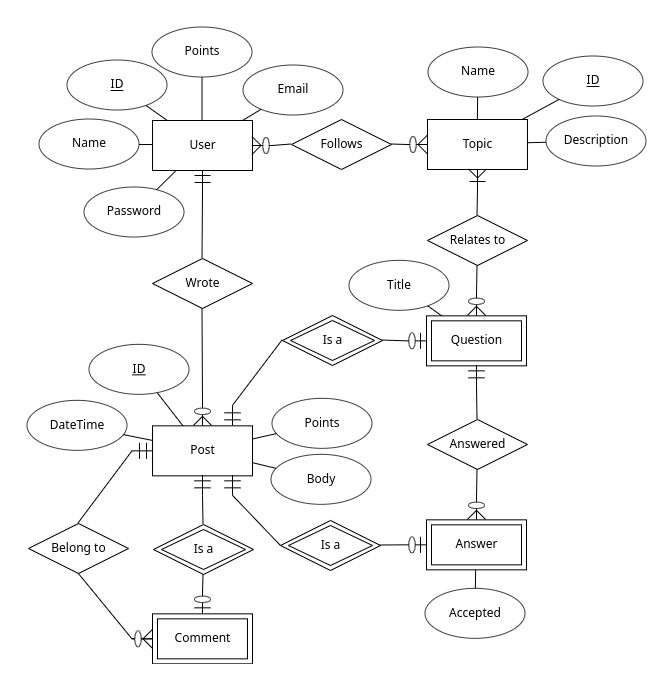
\includegraphics[width=\linewidth]{images/erd1.png}
	\caption{The first design of the ERD}
	\label{erd1}
\end{figure}

However, this may cause inefficiency when retrieving data for any type of post from the database. This is because the attributes of each post would be divided into two tables, requiring us to join the tables to obtain all the data on any particular post.

We therefore tweak the design so that each post type contains all of their fields in the same table, even those that all the post types have in common. This solves the inefficiency because there is no longer a need to join the tables, and this solution still maintains the tables normalized to the same extent that they were prior.

Another consideration we must make is that since a comment is a type of post, and a comment can have child comments, we encounter a cycle in the ERD. Specifically, this means that the depth of a comment thread would have no limit. This can cause issues if we try to query all the descendant comments of any post, since we would need a recursive query for this.

We may consider applying certain techniques such as materialized paths or using a closure table, which would make this kind of query trivial. However, if we give our system some consideration, we can be fairly certain that such queries need not be made.

For example, when the website needs to load all the child comments of any particular question, we are only interested in the top-level comments at first. Retrieving those is also a simple query, since each comment knows its direct parent. Once we have those, the application level can recursively query all the top-level comments of each of those comments, meaning it would obtain all the second-level comments of the question. Similarly, our application can obtain all the comments, regardless of how many levels deep it can be found.

This approach is preferable in our scenario, since obtaining all the descendant comments in one bulk, as techniques like materialized path and closure tables would allow is unhelpful to us. This is because we need to display them in a hierarchical structure, and retrieving them in bulk would then require further processing by the application in order to structure them accordingly.

Another possible modification which we may consider to make the retrieval of comments more efficient is to only allow a single level of comments, or in other words, not allowing for comments to have child comments. However, this would cause a detriment in user experience, as they would be limited to conducting much discussion on some questions or answers.

Therefore we can conclude that the optimal approach would be to maintain the design as we have described above.

Figure \ref{erd2} shows the final design of the entity relationship diagram for the database we are to make for Ask Us. Although the ERD is more complex, it provides the facility to use simpler and more efficient queries to retrieve the data that our system is interested in.

\begin{figure}[p]
	\centering
	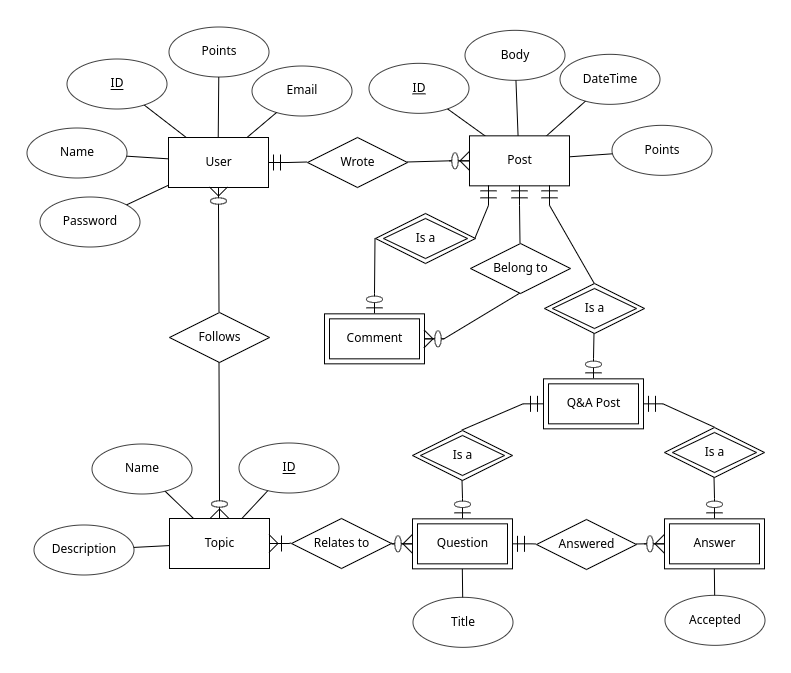
\includegraphics[width=\linewidth]{../../ERD/erd.png}
	\caption{The final ERD for the database for Ask Us}
	\label{erd2}
\end{figure}